% Detailed per-dataset results (REVE-style). Counts filled in from dataset_counts.json.
\section{Detailed Results per Dataset}\label{app:fullmetrics}
Table~\ref{tab:overview} reports balanced accuracy only. Here every dataset is described and
given its own table with the metrics that prior EEG foundation models report: balanced accuracy,
Cohen's $\kappa$ and weighted F1 for every task, and additionally AUROC and AUC-PR for the binary
tasks. All numbers come from the strict linear probe of Sec.~\ref{sec:lpproto}, measured by us
with the released weights on identical samples and splits; balanced accuracy on the validation
split is the only selection criterion (the regularization $C$ and, for REVE, the readout).

\noindent\textbf{Uncertainty.} The external models are released as single checkpoints, so we
evaluate one checkpoint of SpecBraM as well, our main released model, and quantify the
uncertainty of every model in the same way. For mixed-label or multiclass tasks we use ordinary
cluster resampling of test subjects with replacement. For binary tasks whose subjects each
have one true label, subjects are resampled within true-label strata. For TUEV the cluster unit
is the recording, since its evaluation files are anonymized. Candidate resamples missing any
test-set class are discarded until 1{,}000 valid replicates are obtained. Every metric is
recomputed on the pooled samples of the drawn clusters; the 2.5th and 97.5th percentiles form
the nominal 95\% confidence interval. These intervals describe test-cohort sampling variation
conditional on the fitted checkpoint and probe, not pretraining-seed variability. To show the variation of our
pretraining, each table also lists SpecBraM's mean and standard deviation over its three
pretraining seeds; this row is not used for the comparison.

\noindent\textbf{Confusion matrices.} For every dataset we also show the row-normalized confusion
matrices of SpecBraM and of REVE, the strongest baseline, and their difference, to see which
classes each model recognizes.

\noindent\textbf{Paired differences.} Overlapping intervals do not imply that two models are
equivalent, so we also bootstrap the difference itself: on each of the 1{,}000 resamples the
score of every external model is subtracted from SpecBraM's on the same drawn clusters,
preserving the pairing (Table~\ref{tab:paired}). The generated table gives the nominal,
unadjusted 95\% intervals for each difference; no correction for multiple comparisons is
applied. An interval excluding zero is evidence of a difference under this procedure. An
interval containing zero indicates no detected difference, not equivalence or noninferiority.
The intervals condition on the evaluated checkpoints and do not include training variability.
% auto-generated by make_arxiv_tables.py -- do not edit
\begin{table*}[t]\centering\small
\setlength{\tabcolsep}{6pt}
\caption{\textbf{Paired bootstrap of the difference} in balanced accuracy (points) between
SpecBraM's main checkpoint and each external model, computed on the same 1{,}000 resamples of
the test subjects (TUEV: recordings), with its nominal, unadjusted 95\% confidence interval.
Positive: SpecBraM better. Bold: the interval excludes zero; this is not an equivalence test.}
\label{tab:paired}
\begin{tabular}{l ccccc}
\toprule
Dataset & CBraMod & LaBraM-Base & BIOT & CSBrain & REVE-Base\\
\midrule
ISRUC & \ci{\textbf{+6.2}}{+4.28}{+8.01} & \ci{\textbf{+3.8}}{+1.93}{+5.41} & \ci{\textbf{+5.4}}{+2.81}{+8.11} & \ci{\textbf{+6.0}}{+4.85}{+7.11} & \ci{-0.3}{-1.89}{+1.36} \\
HMC & \ci{\textbf{+12.3}}{+9.53}{+15.51} & \ci{\textbf{+11.0}}{+8.45}{+13.63} & \ci{\textbf{+8.4}}{+6.06}{+10.89} & \ci{\textbf{+13.1}}{+9.82}{+16.35} & \ci{\textbf{+3.8}}{+1.83}{+5.90} \\
TUAB & \ci{\textbf{+3.5}}{+1.09}{+6.12} & \ci{\textbf{+3.7}}{+1.52}{+6.06} & -- & \ci{\textbf{+4.1}}{+1.63}{+6.44} & \ci{-0.8}{-2.71}{+1.21} \\
TUEV & \ci{+3.0}{-3.06}{+9.68} & \ci{\textbf{+8.8}}{+1.87}{+15.76} & -- & \ci{-0.9}{-7.48}{+10.32} & \ci{+0.9}{-4.63}{+10.22} \\
MA & \ci{+12.8}{-3.12}{+25.00} & \ci{\textbf{+10.1}}{+5.21}{+13.19} & -- & \ci{\textbf{+22.6}}{+12.50}{+32.29} & \ci{+9.7}{+0.00}{+17.36} \\
Mumtaz & \ci{\textbf{+4.7}}{+0.08}{+11.37} & \ci{\textbf{+6.3}}{+0.90}{+12.38} & -- & \ci{\textbf{+7.6}}{+3.30}{+12.04} & \ci{+3.7}{-6.65}{+17.43} \\
FACED & \ci{\textbf{+5.0}}{+2.48}{+7.52} & \ci{\textbf{+5.3}}{+3.18}{+7.58} & -- & \ci{\textbf{+4.1}}{+0.04}{+8.01} & \ci{+2.1}{-0.70}{+4.58} \\
PhysioNet-MI & \ci{\textbf{+10.5}}{+6.49}{+14.78} & \ci{\textbf{+11.8}}{+8.70}{+14.77} & -- & \ci{\textbf{+11.9}}{+7.68}{+16.51} & \ci{+1.4}{-2.03}{+5.15} \\
\bottomrule
\end{tabular}
\end{table*}


\noindent\textbf{Per-subject comparison.} A higher pooled score could come from a few subjects.
Fig.~\ref{fig:per_subject} compares SpecBraM and REVE subject by subject, and
Table~\ref{tab:per_subject} counts the subjects on which SpecBraM is better, equal or worse than
each external model. SpecBraM is better than CBraMod and CSBrain on every sleep subject and than
LaBraM and BIOT on all but one subject per sleep dataset; on every other dataset it is better than
CBraMod, LaBraM and CSBrain on more subjects than it is worse. Against REVE it is better on $81\%$ of the HMC subjects and on three of the
four MA subjects, and about even on ISRUC, Mumtaz, FACED and PhysioNet-MI. On the clinical
corpora the comparison is close in both directions: REVE is better on slightly more TUAB
patients ($41\%$ vs.\ $36\%$, $23\%$ ties) and SpecBraM on slightly more TUEV recordings ($45\%$
vs.\ $37\%$).
\begin{figure*}[t]\centering
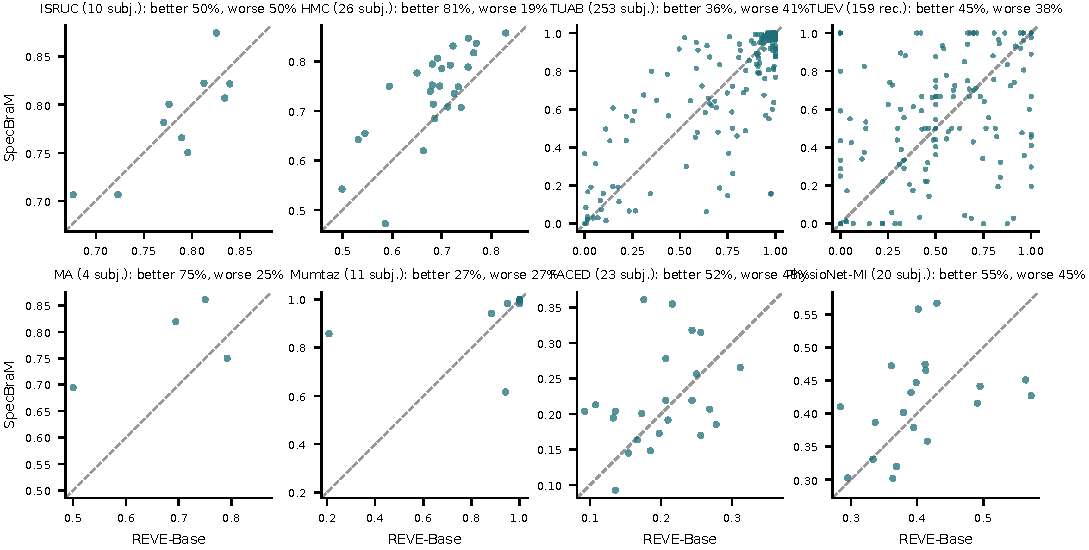
\includegraphics[width=\textwidth]{figures/per_subject.pdf}
\caption{\textbf{Per-subject balanced accuracy}, SpecBraM's main checkpoint vs.\ REVE-Base
(strict linear probe; one point per test subject, TUEV: per recording; dashed: equality).
Titles: share of subjects on which SpecBraM is better / worse.}
\label{fig:per_subject}
\end{figure*}
% auto-generated by make_case_figs.py -- do not edit
\begin{table}[h]\centering\small
\setlength{\tabcolsep}{3pt}
\caption{\textbf{Per-subject comparison}: percentage of test subjects (TUEV: recordings) on
which SpecBraM's balanced accuracy is higher / equal / lower than that of each external model
(strict linear probe, one checkpoint per model).}
\label{tab:per_subject}
\resizebox{\columnwidth}{!}{%
\begin{tabular}{l ccccc}
\toprule
Dataset & CBraMod & LaBraM-Base & BIOT & CSBrain & REVE-Base \\
\midrule
ISRUC (10 subj.) & 100/0/0 & 90/0/10 & 90/0/10 & 100/0/0 & 50/0/50 \\
HMC (26 subj.) & 100/0/0 & 96/0/4 & 96/0/4 & 100/0/0 & 81/0/19 \\
TUAB (253 subj.) & 60/13/27 & 65/10/25 & -- & 62/11/27 & 36/23/41 \\
TUEV (159 rec.) & 50/17/33 & 50/19/31 & -- & 45/21/34 & 45/18/37 \\
MA (4 subj.) & 75/0/25 & 100/0/0 & -- & 100/0/0 & 75/0/25 \\
Mumtaz (11 subj.) & 45/36/19 & 64/27/9 & -- & 82/18/0 & 27/45/28 \\
FACED (23 subj.) & 78/0/22 & 83/0/17 & -- & 65/0/35 & 52/0/48 \\
PhysioNet-MI (20 subj.) & 85/0/15 & 95/0/5 & -- & 90/0/10 & 55/0/45 \\
\bottomrule
\end{tabular}}
\end{table}


\subsection{Sleep Staging: ISRUC}
ISRUC subgroup~I \cite{khalighi2016isruc} contains one overnight polysomnography of each of
100 adults with sleep complaints, scored by experts in 30-s epochs into five AASM stages (W, N1,
N2, N3, REM). We use the six mastoid-referenced EEG leads (F3-A2, C3-A2, O1-A2, F4-A1, C4-A1,
O2-A1; 200\,Hz), of which F3/F4 are missing in some recordings, and the subject split of CBraMod
and CSBrain (subjects 1--80/81--90/91--100; @ISRUC_N@ epochs). A 30-s epoch is represented by
the mean of the features of its three 10-s windows.
% auto-generated by make_arxiv_tables.py -- do not edit
\begin{table}[h]\centering\small
\setlength{\tabcolsep}{3pt}
\caption{\textbf{Detailed results on ISRUC} (strict linear probe). One checkpoint
per model, with the 95\% confidence interval from 1{,}000 bootstrap resamples of the
10 test subjects. Below SpecBraM's main
checkpoint: mean${\pm}$std over its three pretraining seeds. Bold: best per column.}
\label{tab:det_isruc}
\resizebox{\columnwidth}{!}{%
\begin{tabular}{l ccc}
\toprule
Model & Balanced Acc. & Cohen's $\kappa$ & Weighted F1\\
\midrule
\textbf{SpecBraM} & \ci{0.790}{0.764}{0.816} & \ci{0.733}{0.692}{0.773} & \ci{\textbf{0.795}}{0.757}{0.830} \\
\quad{\footnotesize three seeds, mean${\pm}$std} & \val{0.797}{0.006} & \val{0.744}{0.010} & \val{0.803}{0.008} \\
CBraMod & \ci{0.728}{0.702}{0.752} & \ci{0.658}{0.608}{0.705} & \ci{0.734}{0.698}{0.770} \\
LaBraM-Base & \ci{0.752}{0.720}{0.777} & \ci{0.686}{0.642}{0.724} & \ci{0.754}{0.716}{0.787} \\
BIOT & \ci{0.736}{0.691}{0.771} & \ci{0.666}{0.601}{0.715} & \ci{0.740}{0.686}{0.785} \\
CSBrain & \ci{0.730}{0.706}{0.752} & \ci{0.674}{0.638}{0.714} & \ci{0.749}{0.719}{0.782} \\
REVE-Base & \ci{\textbf{0.793}}{0.765}{0.816} & \ci{\textbf{0.736}}{0.703}{0.769} & \ci{\textbf{0.795}}{0.765}{0.824} \\
\bottomrule
\end{tabular}}
\end{table}

\begin{figure}[h]\centering
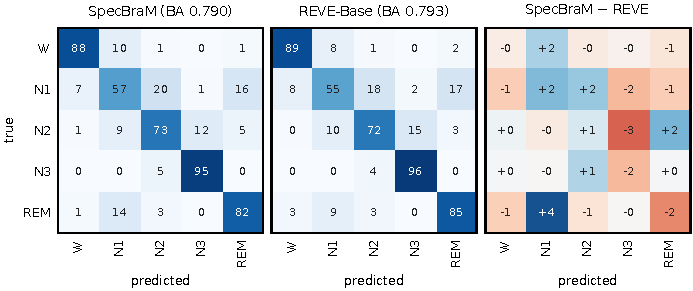
\includegraphics[width=\columnwidth]{figures/cm_isruc.pdf}
\caption{\textbf{Confusion matrices on ISRUC} (strict linear probe, row-normalized recall in \%): SpecBraM's main checkpoint, REVE-Base and their difference (blue: SpecBraM higher).}
\label{fig:cm_isruc}
\end{figure}
Fig.~\ref{fig:cm_isruc}: The two models make the same kinds of errors: N1 is confused with N2 and REM, and N3 with N2. Per-class recall differs by at most $2.4$ points, consistent with the small difference in balanced-accuracy point estimates.

\subsection{Sleep Staging: HMC}
HMC \cite{alvarez2021hmc} contains 151 clinical polysomnographies from the Haaglanden Medisch
Centrum, scored in 30-s epochs into the same five stages. We use the four EEG leads (F4-M1,
C4-M1, O2-M1, C3-M2; 256\,Hz) and the split of CBraMod and CSBrain by sorted subject ID
(100/25/26 recordings; @HMC_N@ epochs). Epochs are represented as for ISRUC.
% auto-generated by make_arxiv_tables.py -- do not edit
\begin{table}[h]\centering\small
\setlength{\tabcolsep}{3pt}
\caption{\textbf{Detailed results on HMC} (strict linear probe). One checkpoint
per model, with the 95\% confidence interval from 1{,}000 bootstrap resamples of the
26 test subjects. Below SpecBraM's main
checkpoint: mean${\pm}$std over its three pretraining seeds. Bold: best per column.}
\label{tab:det_hmc}
\resizebox{\columnwidth}{!}{%
\begin{tabular}{l ccc}
\toprule
Model & Balanced Acc. & Cohen's $\kappa$ & Weighted F1\\
\midrule
\textbf{SpecBraM} & \ci{\textbf{0.742}}{0.699}{0.776} & \ci{\textbf{0.675}}{0.620}{0.724} & \ci{\textbf{0.751}}{0.707}{0.791} \\
\quad{\footnotesize three seeds, mean${\pm}$std} & \val{0.743}{0.002} & \val{0.675}{0.002} & \val{0.749}{0.003} \\
CBraMod & \ci{0.619}{0.576}{0.654} & \ci{0.513}{0.459}{0.567} & \ci{0.619}{0.572}{0.665} \\
LaBraM-Base & \ci{0.632}{0.583}{0.673} & \ci{0.530}{0.473}{0.585} & \ci{0.636}{0.586}{0.680} \\
BIOT & \ci{0.658}{0.609}{0.697} & \ci{0.562}{0.507}{0.615} & \ci{0.661}{0.616}{0.704} \\
CSBrain & \ci{0.611}{0.580}{0.641} & \ci{0.515}{0.472}{0.554} & \ci{0.625}{0.590}{0.660} \\
REVE-Base & \ci{0.704}{0.664}{0.737} & \ci{0.623}{0.577}{0.670} & \ci{0.707}{0.671}{0.745} \\
\bottomrule
\end{tabular}}
\end{table}

\begin{figure}[h]\centering
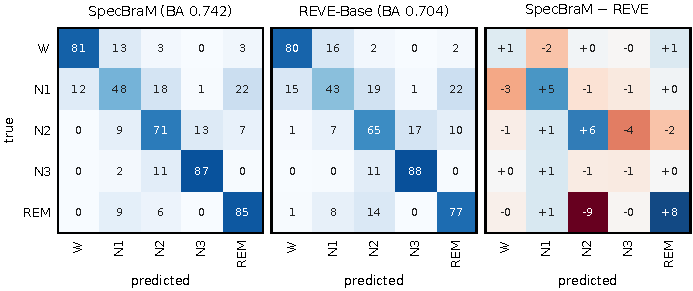
\includegraphics[width=\columnwidth]{figures/cm_hmc.pdf}
\caption{\textbf{Confusion matrices on HMC} (strict linear probe, row-normalized recall in \%): SpecBraM's main checkpoint, REVE-Base and their difference (blue: SpecBraM higher).}
\label{fig:cm_hmc}
\end{figure}
Fig.~\ref{fig:cm_hmc}: SpecBraM's lead over REVE comes from the transitional and REM stages: its recall is higher by $5.0$ points for N1, $6.0$ for N2 and $7.7$ for REM, while W and N3, the stages with the most distinct spectra, are recognized equally well by both.

\noindent\textbf{Case study: one night per dataset.} Fig.~\ref{fig:hypnogram} shows the
hypnograms of one test subject per sleep dataset, chosen by rule as the subject whose SpecBraM
balanced accuracy is closest to the median of its dataset, with the stages predicted by
SpecBraM, REVE and CBraMod from the frozen features of each 30-s epoch alone (no sequence
model). All models follow the sleep cycles; their errors concentrate at stage transitions and in
N1. On the ISRUC night the three models are close (balanced accuracy $0.800$, $0.776$ and $0.728$).
On the HMC night SpecBraM reaches $0.750$ against $0.594$ for REVE, which scores almost a third
of the N2 epochs as N3 (99 of 319 vs.\ 27 for SpecBraM) and half of the REM epochs as N2 (69 of
132 vs.\ 12), the same errors that dominate REVE's confusion matrix on the whole dataset
(Fig.~\ref{fig:cm_hmc}).
\begin{figure*}[t]\centering
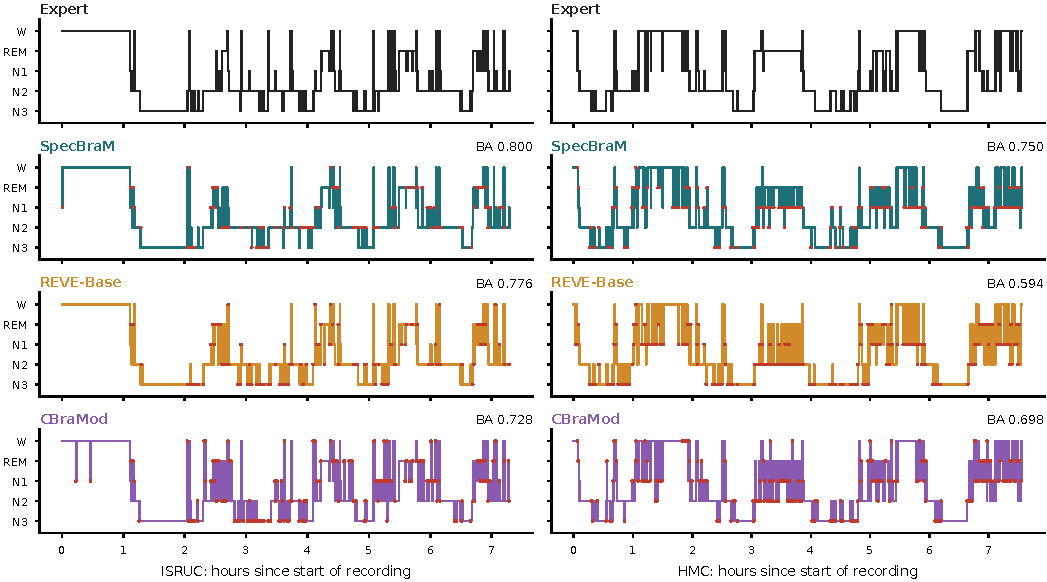
\includegraphics[width=\textwidth]{figures/hypnogram.pdf}
\caption{\textbf{Whole-night hypnograms} of one test subject per sleep dataset (left: ISRUC,
right: HMC; the subject whose SpecBraM balanced accuracy is closest to the dataset median).
Top: expert scoring; below: stages predicted by the strict linear probe on each model's frozen
features, epoch by epoch. Red dots: errors.}
\label{fig:hypnogram}
\end{figure*}

\subsection{Abnormal EEG Detection: TUAB}
TUAB \cite{obeid2016tuh} contains clinical EEG recordings of the Temple University Hospital
labeled normal or abnormal by neurologists. Following CBraMod, recordings are resampled to
200\,Hz, filtered (0.3--75\,Hz, 60\,Hz notch), converted to 16 bipolar channels of the TCP
montage and cut into non-overlapping 10-s windows that inherit the recording label. The official
evaluation folder is the test set; the training folder is split 80/20 by sorted patient ID
within each class (@TUAB_N@ windows). The prepared metadata show three patients shared
between training and validation under this original per-class split. Test patients are disjoint
from both training and validation. All models use these same samples and splits; the overlap
limits validation independence. This downstream split issue is separate from possible TUEG
pretraining overlap.
% auto-generated by make_arxiv_tables.py -- do not edit
\begin{table*}[t]\centering\small
\setlength{\tabcolsep}{8pt}
\caption{\textbf{Detailed results on TUAB} (strict linear probe). One checkpoint
per model, with the 95\% confidence interval from 1{,}000 bootstrap resamples of the
253 test subjects. Below SpecBraM's main
checkpoint: mean${\pm}$std over its three pretraining seeds. Bold: best per column.}
\label{tab:det_tuab}

\begin{tabular}{l ccccc}
\toprule
Model & Balanced Acc. & Cohen's $\kappa$ & Weighted F1 & AUROC & AUC-PR\\
\midrule
\textbf{SpecBraM} & \ci{0.813}{0.775}{0.850} & \ci{0.627}{0.554}{0.700} & \ci{0.815}{0.778}{0.851} & \ci{\textbf{0.891}}{0.851}{0.924} & \ci{0.897}{0.860}{0.929} \\
\quad{\footnotesize three seeds, mean${\pm}$std} & \val{0.805}{0.007} & \val{0.611}{0.014} & \val{0.807}{0.007} & \val{0.880}{0.011} & \val{0.890}{0.008} \\
CBraMod & \ci{0.778}{0.738}{0.814} & \ci{0.558}{0.480}{0.629} & \ci{0.780}{0.742}{0.816} & \ci{0.856}{0.810}{0.894} & \ci{0.857}{0.812}{0.893} \\
LaBraM-Base & \ci{0.776}{0.740}{0.812} & \ci{0.554}{0.484}{0.624} & \ci{0.779}{0.744}{0.814} & \ci{0.856}{0.817}{0.891} & \ci{0.851}{0.806}{0.889} \\
CSBrain & \ci{0.772}{0.736}{0.805} & \ci{0.546}{0.475}{0.611} & \ci{0.774}{0.740}{0.807} & \ci{0.845}{0.804}{0.882} & \ci{0.836}{0.786}{0.878} \\
REVE-Base & \ci{\textbf{0.821}}{0.781}{0.861} & \ci{\textbf{0.644}}{0.565}{0.722} & \ci{\textbf{0.823}}{0.784}{0.861} & \ci{0.889}{0.848}{0.925} & \ci{\textbf{0.902}}{0.864}{0.933} \\
\bottomrule
\end{tabular}
\end{table*}

\begin{figure}[h]\centering
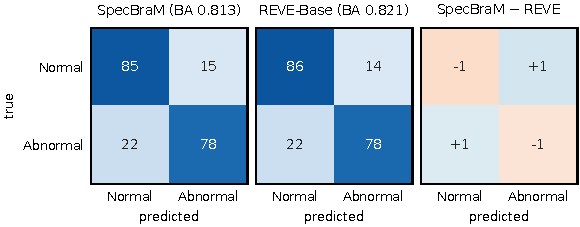
\includegraphics[width=\columnwidth]{figures/cm_tuab.pdf}
\caption{\textbf{Confusion matrices on TUAB} (strict linear probe, row-normalized recall in \%): SpecBraM's main checkpoint, REVE-Base and their difference (blue: SpecBraM higher).}
\label{fig:cm_tuab}
\end{figure}
Fig.~\ref{fig:cm_tuab}: Both models recognize normal and abnormal recordings almost equally well (recall within one point of each other); REVE's slightly higher balanced accuracy is spread over both classes.

\subsection{Event Classification: TUEV}
TUEV \cite{obeid2016tuh} annotates clinical EEG with six event classes: spike and sharp wave
(SPSW), generalized and lateralized periodic epileptiform discharges (GPED, PLED), eye movement
(EYEM), artifact (ARTF) and background (BCKG). Following CBraMod, each annotated 1-s event is
represented by a 5-s window centred on it, with the same filtering and 16-channel bipolar
montage as TUAB. The official evaluation folder is the test set and the training folder is split
80/20 by sorted patient ID (@TUEV_N@ windows), with no patient overlap among the three
downstream splits. Background makes up 65\% of the windows; Cohen's
$\kappa$ and weighted F1 are dominated by it, whereas balanced accuracy weights the rare
epileptiform classes equally. This explains why REVE has the highest $\kappa$ and weighted F1
here although its balanced accuracy is below SpecBraM's and CSBrain's.
% auto-generated by make_arxiv_tables.py -- do not edit
\begin{table}[h]\centering\small
\setlength{\tabcolsep}{3pt}
\caption{\textbf{Detailed results on TUEV} (strict linear probe). One checkpoint
per model, with the 95\% confidence interval from 1{,}000 bootstrap resamples of the
159 test recordings. Below SpecBraM's main
checkpoint: mean${\pm}$std over its three pretraining seeds. Bold: best per column.}
\label{tab:det_tuev}
\resizebox{\columnwidth}{!}{%
\begin{tabular}{l ccc}
\toprule
Model & Balanced Acc. & Cohen's $\kappa$ & Weighted F1\\
\midrule
\textbf{SpecBraM} & \ci{0.555}{0.491}{0.648} & \ci{0.467}{0.369}{0.557} & \ci{0.722}{0.659}{0.777} \\
\quad{\footnotesize three seeds, mean${\pm}$std} & \val{0.561}{0.025} & \val{0.474}{0.049} & \val{0.724}{0.027} \\
CBraMod & \ci{0.525}{0.471}{0.609} & \ci{0.399}{0.327}{0.480} & \ci{0.669}{0.598}{0.742} \\
LaBraM-Base & \ci{0.468}{0.416}{0.545} & \ci{0.327}{0.228}{0.423} & \ci{0.624}{0.518}{0.710} \\
CSBrain & \ci{\textbf{0.564}}{0.505}{0.621} & \ci{0.421}{0.348}{0.489} & \ci{0.683}{0.619}{0.745} \\
REVE-Base & \ci{0.546}{0.500}{0.587} & \ci{\textbf{0.566}}{0.439}{0.655} & \ci{\textbf{0.778}}{0.727}{0.820} \\
\bottomrule
\end{tabular}}
\end{table}

\begin{figure}[h]\centering
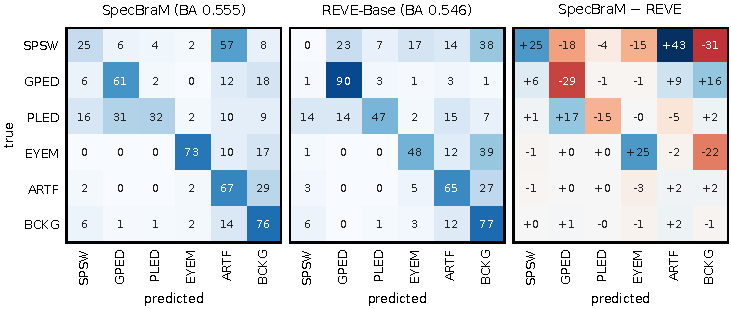
\includegraphics[width=\columnwidth]{figures/cm_tuev.pdf}
\caption{\textbf{Confusion matrices on TUEV} (strict linear probe, row-normalized recall in \%): SpecBraM's main checkpoint, REVE-Base and their difference (blue: SpecBraM higher).}
\label{fig:cm_tuev}
\end{figure}
Fig.~\ref{fig:cm_tuev}: The two models differ in kind. SpecBraM detects spike and sharp waves
(SPSW recall $25\%$ vs.\ $0\%$; REVE never predicts this class) and eye movements ($73\%$ vs.\
$48\%$), events with a distinct spectral signature. REVE is better on the periodic discharges
(GPED $90\%$ vs.\ $61\%$, PLED $47\%$ vs.\ $32\%$), which involve waveform shape and repetition
over seconds. This pattern is consistent with P4, but the models also differ in architecture
and pretraining data, so it does not isolate the effect of phase invariance.

\noindent\textbf{Examples.} Fig.~\ref{fig:tuev_cases} shows four test windows on which the two
models disagree, chosen by rule: for each class, the window that the correct model classifies
with the highest confidence. SpecBraM recognizes a spike and sharp wave that REVE labels as a
lateralized periodic discharge, and an eye-movement window that REVE labels as background. REVE
recognizes a generalized and a lateralized periodic discharge that SpecBraM labels as
background. In the GPED window the discharges recur about every two seconds across all
channels. Their waveform and repetition extend beyond the band power of a single 0.78-s patch.
The patch-local target does not directly supervise this longer temporal pattern (P4), although
the encoder can still represent temporal and waveform information.
\begin{figure*}[t]\centering
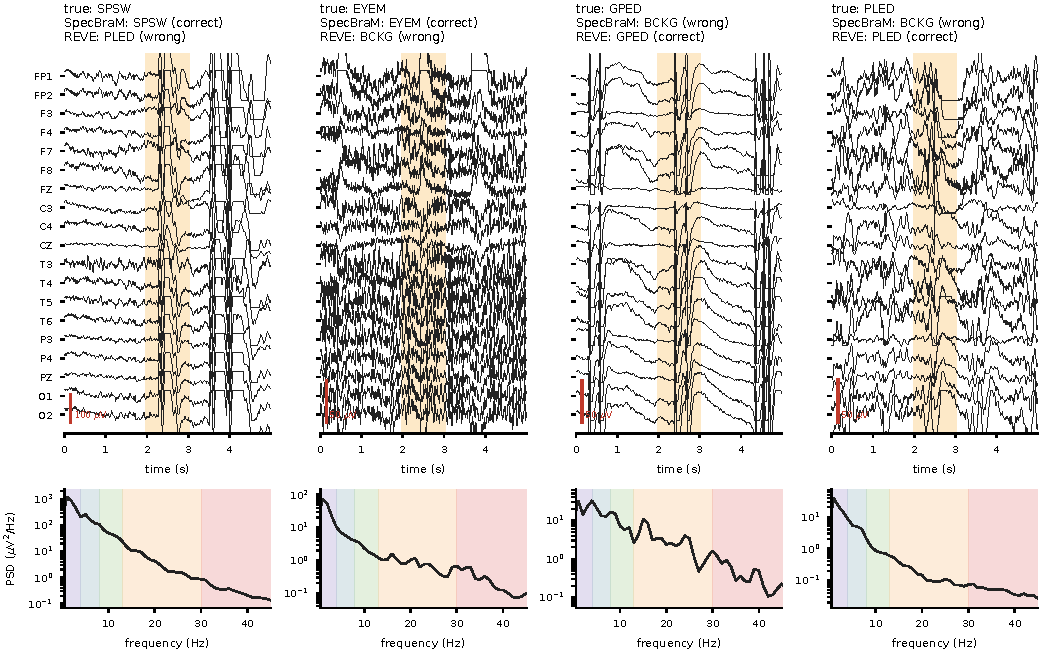
\includegraphics[width=\textwidth]{figures/tuev_cases.pdf}
\caption{\textbf{TUEV examples on which SpecBraM and REVE disagree} (strict linear probe; for
each class the window that the correct model classifies most confidently). Top: the 5-s window
(19 monopolar leads, CBraMod's preprocessing; shaded: the annotated 1-s event; traces clipped to
their row). Bottom: power spectral density averaged over channels, with the five bands of the
target.}
\label{fig:tuev_cases}
\end{figure*}

\subsection{Mental Workload: MA}
The mental arithmetic dataset \cite{zyma2019mentalarith} records 36 subjects at rest and during
serial subtraction with 20 leads (19 standard 10--20 leads and A2-A1; 500\,Hz). Following
CBraMod, recordings are resampled to 200\,Hz and cut into 5-s windows labeled rest or task, and
the sorted subjects are split 28/4/4 (@MA_N@ windows). With four test subjects, MA has by far
the widest confidence intervals of all tasks.
% auto-generated by make_arxiv_tables.py -- do not edit
\begin{table*}[t]\centering\small
\setlength{\tabcolsep}{8pt}
\caption{\textbf{Detailed results on MA} (strict linear probe). One checkpoint
per model, with the 95\% confidence interval from 1{,}000 bootstrap resamples of the
4 test subjects. Below SpecBraM's main
checkpoint: mean${\pm}$std over its three pretraining seeds. Bold: best per column.}
\label{tab:det_ma}

\begin{tabular}{l ccccc}
\toprule
Model & Balanced Acc. & Cohen's $\kappa$ & Weighted F1 & AUROC & AUC-PR\\
\midrule
\textbf{SpecBraM} & \ci{\textbf{0.781}}{0.722}{0.840} & \ci{\textbf{0.583}}{0.526}{0.655} & \ci{\textbf{0.846}}{0.817}{0.876} & \ci{\textbf{0.912}}{0.878}{0.981} & \ci{\textbf{0.783}}{0.751}{0.942} \\
\quad{\footnotesize three seeds, mean${\pm}$std} & \val{0.747}{0.030} & \val{0.500}{0.093} & \val{0.810}{0.047} & \val{0.861}{0.052} & \val{0.706}{0.108} \\
CBraMod & \ci{0.653}{0.507}{0.799} & \ci{0.256}{0.011}{0.510} & \ci{0.686}{0.525}{0.811} & \ci{0.708}{0.532}{0.884} & \ci{0.515}{0.305}{0.730} \\
LaBraM-Base & \ci{0.681}{0.597}{0.736} & \ci{0.342}{0.205}{0.452} & \ci{0.746}{0.700}{0.793} & \ci{0.734}{0.649}{0.834} & \ci{0.571}{0.432}{0.724} \\
CSBrain & \ci{0.556}{0.403}{0.653} & \ci{0.095}{-0.175}{0.275} & \ci{0.626}{0.543}{0.711} & \ci{0.586}{0.402}{0.747} & \ci{0.306}{0.218}{0.451} \\
REVE-Base & \ci{0.684}{0.562}{0.771} & \ci{0.361}{0.143}{0.551} & \ci{0.758}{0.679}{0.838} & \ci{0.757}{0.669}{0.924} & \ci{0.587}{0.485}{0.802} \\
\bottomrule
\end{tabular}
\end{table*}

\begin{figure}[h]\centering
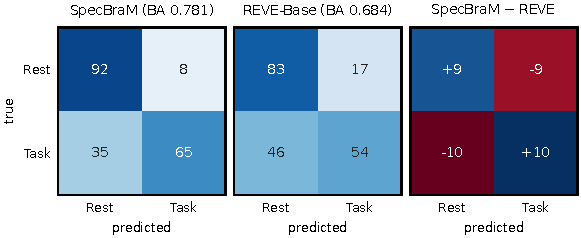
\includegraphics[width=\columnwidth]{figures/cm_ma.pdf}
\caption{\textbf{Confusion matrices on MA} (strict linear probe, row-normalized recall in \%): SpecBraM's main checkpoint, REVE-Base and their difference (blue: SpecBraM higher).}
\label{fig:cm_ma}
\end{figure}
Fig.~\ref{fig:cm_ma}: SpecBraM is better on both conditions (rest $+9.0$, task $+10.4$ points recall), so its lead is not a shift of the decision threshold.

\subsection{Depression: Mumtaz}
Mumtaz \cite{mumtaz2016mdd} contains resting-state EEG (eyes open and closed) of patients with
major depressive disorder and healthy controls, recorded with 19 linked-ear-referenced leads at
256\,Hz. Following CBraMod, recordings are resampled to 200\,Hz, filtered (0.3--75\,Hz, 50\,Hz
notch) and cut into 5-s windows that inherit the subject's diagnosis; recordings are split by
subject within each group (@MUMTAZ_N@ windows).
% auto-generated by make_arxiv_tables.py -- do not edit
\begin{table*}[t]\centering\small
\setlength{\tabcolsep}{8pt}
\caption{\textbf{Detailed results on Mumtaz} (strict linear probe). One checkpoint
per model, with the 95\% confidence interval from 1{,}000 bootstrap resamples of the
11 test subjects. Below SpecBraM's main
checkpoint: mean${\pm}$std over its three pretraining seeds. Bold: best per column.}
\label{tab:det_mumtaz}

\begin{tabular}{l ccccc}
\toprule
Model & Balanced Acc. & Cohen's $\kappa$ & Weighted F1 & AUROC & AUC-PR\\
\midrule
\textbf{SpecBraM} & \ci{\textbf{0.939}}{0.868}{0.995} & \ci{\textbf{0.879}}{0.733}{0.991} & \ci{\textbf{0.940}}{0.865}{0.995} & \ci{\textbf{0.991}}{0.964}{1.000} & \ci{\textbf{0.991}}{0.967}{1.000} \\
\quad{\footnotesize three seeds, mean${\pm}$std} & \val{0.942}{0.007} & \val{0.884}{0.015} & \val{0.942}{0.007} & \val{0.994}{0.003} & \val{0.994}{0.003} \\
CBraMod & \ci{0.893}{0.760}{0.988} & \ci{0.787}{0.513}{0.978} & \ci{0.893}{0.744}{0.989} & \ci{0.973}{0.911}{1.000} & \ci{0.973}{0.908}{1.000} \\
LaBraM-Base & \ci{0.876}{0.744}{0.986} & \ci{0.754}{0.484}{0.974} & \ci{0.877}{0.735}{0.987} & \ci{0.963}{0.882}{0.999} & \ci{0.960}{0.874}{0.999} \\
CSBrain & \ci{0.864}{0.774}{0.943} & \ci{0.727}{0.549}{0.887} & \ci{0.864}{0.772}{0.944} & \ci{0.947}{0.878}{0.990} & \ci{0.942}{0.862}{0.987} \\
REVE-Base & \ci{0.902}{0.743}{0.994} & \ci{0.804}{0.481}{0.989} & \ci{0.901}{0.728}{0.995} & \ci{0.968}{0.879}{1.000} & \ci{0.963}{0.861}{1.000} \\
\bottomrule
\end{tabular}
\end{table*}

\begin{figure}[h]\centering
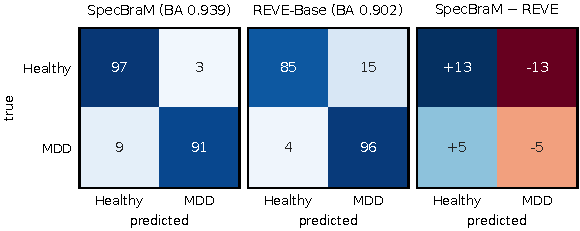
\includegraphics[width=\columnwidth]{figures/cm_mumtaz.pdf}
\caption{\textbf{Confusion matrices on Mumtaz} (strict linear probe, row-normalized recall in \%): SpecBraM's main checkpoint, REVE-Base and their difference (blue: SpecBraM higher).}
\label{fig:cm_mumtaz}
\end{figure}
Fig.~\ref{fig:cm_mumtaz}: SpecBraM's gain comes from fewer healthy subjects classified as depressed (recall of the healthy class $+12.6$ points), at a cost of $5.2$ points on the depressed class.

\subsection{Emotion Recognition: FACED}
FACED \cite{chen2023faced} records 123 subjects watching 28 video clips that elicit nine emotion
categories (anger, disgust, fear, sadness, neutral, amusement, inspiration, joy, tenderness),
with 32 leads at 250\,Hz. The last 30\,s of each clip are resampled to 200\,Hz and cut into three
10-s windows labeled with the clip's category; the sorted subjects are split 80/20/23
(@FACED_N@ windows; chance level $1/9$).
% auto-generated by make_arxiv_tables.py -- do not edit
\begin{table}[h]\centering\small
\setlength{\tabcolsep}{3pt}
\caption{\textbf{Detailed results on FACED} (strict linear probe). One checkpoint
per model, with the 95\% confidence interval from 1{,}000 bootstrap resamples of the
23 test subjects. Below SpecBraM's main
checkpoint: mean${\pm}$std over its three pretraining seeds. Bold: best per column.}
\label{tab:det_faced}
\resizebox{\columnwidth}{!}{%
\begin{tabular}{l ccc}
\toprule
Model & Balanced Acc. & Cohen's $\kappa$ & Weighted F1\\
\midrule
\textbf{SpecBraM} & \ci{\textbf{0.221}}{0.195}{0.248} & \ci{\textbf{0.126}}{0.096}{0.155} & \ci{\textbf{0.219}}{0.193}{0.245} \\
\quad{\footnotesize three seeds, mean${\pm}$std} & \val{0.216}{0.013} & \val{0.119}{0.015} & \val{0.214}{0.010} \\
CBraMod & \ci{0.171}{0.156}{0.188} & \ci{0.069}{0.052}{0.087} & \ci{0.167}{0.151}{0.182} \\
LaBraM-Base & \ci{0.167}{0.152}{0.181} & \ci{0.064}{0.047}{0.079} & \ci{0.163}{0.144}{0.177} \\
CSBrain & \ci{0.179}{0.161}{0.199} & \ci{0.077}{0.057}{0.098} & \ci{0.171}{0.153}{0.189} \\
REVE-Base & \ci{0.200}{0.179}{0.225} & \ci{0.101}{0.076}{0.130} & \ci{0.200}{0.177}{0.224} \\
\bottomrule
\end{tabular}}
\end{table}

\begin{figure*}[t]\centering
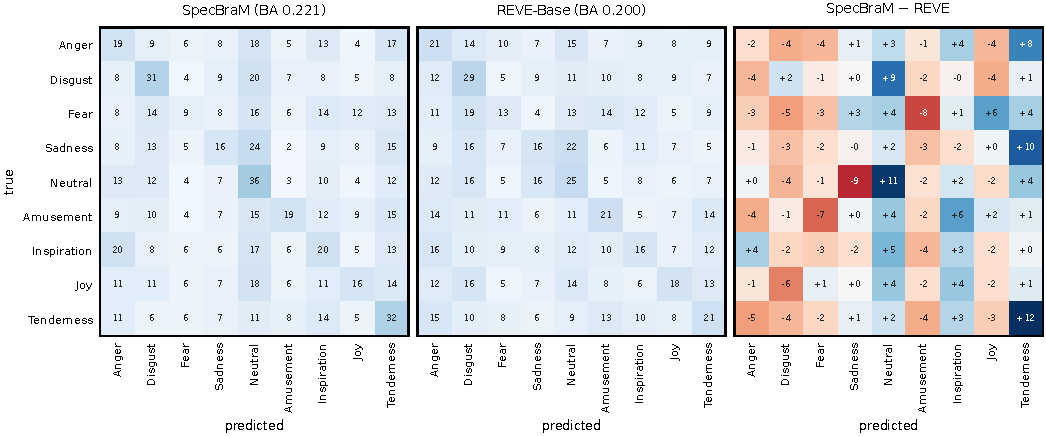
\includegraphics[width=\textwidth]{figures/cm_faced.pdf}
\caption{\textbf{Confusion matrices on FACED} (strict linear probe, row-normalized recall in \%): SpecBraM's main checkpoint, REVE-Base and their difference (blue: SpecBraM higher).}
\label{fig:cm_faced}
\end{figure*}
Fig.~\ref{fig:cm_faced}: Both models are far from perfect on nine emotions. SpecBraM's gain is concentrated on neutral ($+11.2$ points) and tenderness ($+11.6$), the two categories at the low-arousal end, while the other categories differ by a few points in either direction.

\subsection{Motor Imagery: PhysioNet-MI}
PhysioNet-MI \cite{schalk2004bci2000} records 109 subjects with 64 leads at 160\,Hz while they
imagine opening and closing the left fist, the right fist, both fists or both feet. Following
CBraMod, the imagery runs are high-pass filtered at 0.3\,Hz, notch filtered at 60\,Hz and
resampled to 200\,Hz, and the 4-s window after each cue is labeled with the imagined movement;
the sorted subjects are split 70/19/20 (@PHYSIO_N@ windows; chance level $1/4$).
% auto-generated by make_arxiv_tables.py -- do not edit
\begin{table}[h]\centering\small
\setlength{\tabcolsep}{3pt}
\caption{\textbf{Detailed results on PhysioNet-MI} (strict linear probe). One checkpoint
per model, with the 95\% confidence interval from 1{,}000 bootstrap resamples of the
20 test subjects. Below SpecBraM's main
checkpoint: mean${\pm}$std over its three pretraining seeds. Bold: best per column.}
\label{tab:det_physio}
\resizebox{\columnwidth}{!}{%
\begin{tabular}{l ccc}
\toprule
Model & Balanced Acc. & Cohen's $\kappa$ & Weighted F1\\
\midrule
\textbf{SpecBraM} & \ci{\textbf{0.417}}{0.384}{0.450} & \ci{\textbf{0.223}}{0.179}{0.267} & \ci{\textbf{0.416}}{0.383}{0.449} \\
\quad{\footnotesize three seeds, mean${\pm}$std} & \val{0.397}{0.018} & \val{0.196}{0.024} & \val{0.396}{0.018} \\
CBraMod & \ci{0.312}{0.286}{0.340} & \ci{0.083}{0.048}{0.119} & \ci{0.310}{0.282}{0.337} \\
LaBraM-Base & \ci{0.299}{0.285}{0.314} & \ci{0.065}{0.047}{0.085} & \ci{0.299}{0.282}{0.312} \\
CSBrain & \ci{0.298}{0.273}{0.325} & \ci{0.064}{0.030}{0.100} & \ci{0.295}{0.270}{0.320} \\
REVE-Base & \ci{0.403}{0.371}{0.438} & \ci{0.204}{0.161}{0.250} & \ci{0.403}{0.371}{0.437} \\
\bottomrule
\end{tabular}}
\end{table}

\begin{figure}[h]\centering
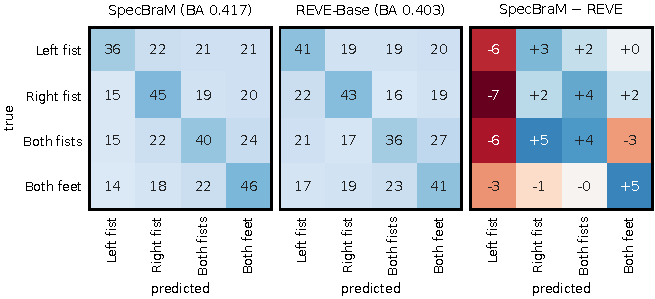
\includegraphics[width=\columnwidth]{figures/cm_physio.pdf}
\caption{\textbf{Confusion matrices on PhysioNet-MI} (strict linear probe, row-normalized recall in \%): SpecBraM's main checkpoint, REVE-Base and their difference (blue: SpecBraM higher).}
\label{fig:cm_physio}
\end{figure}
Fig.~\ref{fig:cm_physio}: SpecBraM is better on bilateral imagery (both fists $+4.2$, both feet $+4.9$ points) and slightly worse on the left fist ($-5.5$); distinguishing the left and right fist requires lateralized spatial patterns that a mean-pooled readout dilutes.
